\chapter{Questions difficulty}
During the first pilot family and friends were asked to play the game and provide feedback. With the help of the 83 games played, we were able to get information about some important aspects of the game: which questions are selected by the users, are they answering randomly or by thinking, how much time they take to answer the questions. This feedback was really useful to understand how difficult the game was and what kind of improvement has to be made. More analysis about this pilot will be done in section \ref{sec:pilot1}. One of the first issue was that the questions were generated completely randomly and there was no concern about how difficult they were, we mostly used parameters that we thought would make sense and not too difficult. We had two main reasons for wanting to be able to change the difficulty at will.\\
The first and most obvious reason is that it makes the game more enjoyable, getting hard questions and failing over and over is  not amusing and the same goes if you only get easy question which offer no challenge at all. The second reason is that by being able to toy with the difficulty, we can test hypotheses and improve our understanding of memory: if we think that some parameter is a central part of what makes an element memorable we can then consider it when modifying questions' difficulty and see whether or not this affects the results when games are played.\\\\
It was therefore important to add some modularity to the question generation process and decide what parameters could be played with to influence the difficulty. Note that older events are obviously harder than recent events so we did not take into account the creation date of a post when discussing the difficulty of a question. We approached the problem from two angles, the selection of items and the generation of the question itself.\\\\
Some items will be harder to remember than others no matter the way the question is then generated. For instance, finding out precisely when something was posted is hard if it is in the middle of a lot of other posts because it was posted during a period of heavy usage of Facebook. On the other hand, isolated posts are really memorable because they are often about something so noteworthy that it made the user go on Facebook and talk about it when they were in the middle of a low usage period.\\\\
The way items are used when generating questions is also something that increases and decreases difficulty. The choice of other alternatives in a multiple choice questions has a lot of influence on the difficulty and the size of the proposed time periods on a time question has also an influence.

\section{Clustering}
\subsection{Why do we need clustering}
Clustering is a standard data analysis technique. ``[It] is the task of grouping a set of objects in such a way that objects in the same group (called a cluster) are more similar (in some sense or another) to each other than to those in other groups (clusters).''\cite{clustering} It is often used in data mining to perform pattern recognition as it allows to find similar items in a data set. The reason we are using it is that we want to find sets of similar posts or similar pages which are then hard to compare to each other. This is of great help when generating ordering questions as three elements belonging to a same cluster are then harder to order than those in different clusters.
\subsection{Algorithm choice}
There are a lot of different algorithms which can achieve clustering. They all have different behaviors and required inputs. Some of the most common algorithms are k-means and DBSCAN.\\
K-means ``aims to partition $n$ observations into $k$ clusters in which each observation belongs to the cluster with the nearest mean''\cite{kmeans}. The algorithm works quite well when the number of clusters is known in advance and provides a centroid for each cluster, which is the mean value for each cluster.\\
``Density-based spatial clustering of applications with noise (DBSCAN) [...] groups together points that are closely packed together (points with many nearby neighbors), marking as outliers points that lie alone in low-density regions (whose nearest neighbors are too far away).''\cite{dbscan} This algorithm does not provide centroids but has the nice property to discover the right number of cluster by itself based on the density distribution of the dataset.\\\\
Figure \ref{fig:clustComp} shows a visual representation of the results of different variations of k-means and DBSCAN when applied to the same datasets. One can see that k-means works well when the number of expected clusters is the same as the number of clusters that the data set actually has. However, when the data set has a different number of cluster or their shape is such that one cannot enclose them in separate circles, the results are less than convincing. On the other hand DBSCAN behaves well in all those cases.\\
In our application, we do not know the number of clusters in advance, it is something we would like the algorithm to help us discover, therefore the choice was to use DBSCAN.

\begin{figure}
\centering
{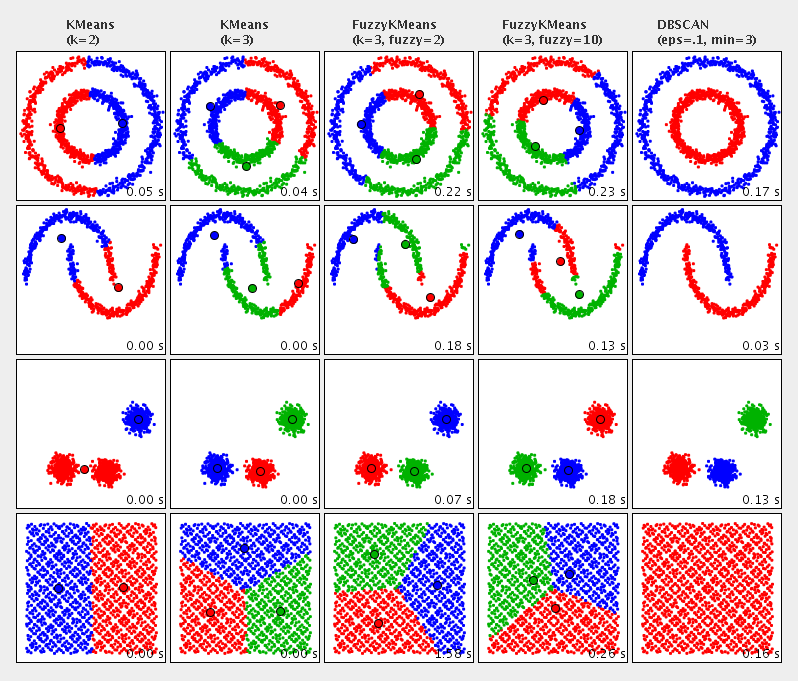
\includegraphics[width=6in]{images/cluster_comparison.png}}
\caption{Comparison of multiple clustering techniques from the Apache maths Commons documentation\cite{apachecluster}}
\label{fig:clustComp}
\end{figure}
\newcommand\minpts{\mathit{minPts}}
\section{How does DBSCAN work}
\subsection{General notions}
Besides the data set, DBSCAN works with two parameters as inputs, $\epsilon$ and $\minpts$. $\epsilon$ can be seen as a density measure, it is the distance between two points which we would consider acceptable for them to be in the same cluster. $\minpts$ is the minimum number of points in a cluster.\\
Let's introduce a few notions\cite{dbscan}:
\begin{itemize}
	\item A \emph{core point} is a point which is surrounded by at least $\minpts$ points within a distance of $\epsilon$. Those points are said to be \emph{directly reachable} from this \emph{core point}. By definition, no point is \emph{directly reachable} from a non-core point.
	\item A point $q$ is said to be \emph{reachable} from a core point $p$ if there exists a sequence of points, all \emph{directly reachable} from the previous one, which starts at $p$ and ends at $q$. All those points must be \emph{core points} except $q$.
	\item All non-core, non-reachable points are \emph{outliers}
	\item Two points $p$ and $q$ are \emph{density connected} if there is a point $o$ from which they are both \emph{reachable}
\end{itemize}

And then the points in a cluster satisfy the following properties\cite{dbscan}:
\begin{itemize}
	\item All points within the cluster are mutually density-connected.
	\item If a point is \emph{reachable} from any point in a cluster, it is part of the cluster as well.
\end{itemize}

Figure \ref{fig:reachExample} illustrates those definitions.

\begin{figure}
\centering
{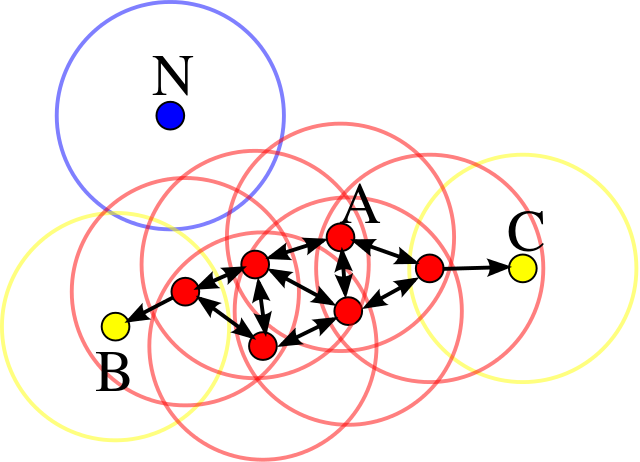
\includegraphics[width=3.5in]{images/reach_example.png}}
\caption{This figure taken from the Wikipedia article on DBSCAN \cite{dbscan} shows an example where $\minpts=4$. $\epsilon$ is represented by the circles. The points in red are \emph{core points}, the ones in yellow are \emph{reachable} and the one in blue is an outlier. The cluster would be comprised of points in red and yellow.}
\label{fig:reachExample}
\end{figure}

\subsection{The algorithm itself}

Let's first define the $\epsilon$-\emph{neighborhood} of a point as the set of points which are at a distance less than $\epsilon$ from this point. The algorithm works as follows\cite{dbscan}:
\begin{enumerate}
	\item \label{initdbscan} Pick a point $P$ from the dataset that was not visited yet and mark $P$ as visited. If no such point exists, the algorithm is completed.
	\item Let $N$ be the $\epsilon$-\emph{neighborhood} of this point. If $N$ contains at least $\minpts$ points, $P$ is a \emph{core point}. In that case create a new cluster $C$ containing only $P$ and carry on to \ref{preloopdbscan}, otherwise go back to \ref{initdbscan}.
	\item\label{preloopdbscan} All the points in $N$ should obviously be part of cluster $C$ as they are neighbors of a \emph{core point} ($P$) and are at a distance less than $\epsilon$ from this point. We must include them in the cluster, but if those points are also \emph{core points} we must also include their neighborhoods and so on (forming sequences of \emph{core points} to find all the \emph{reachable} points). To achieve this, we will put all the points we have to visit in a set we will call $V$. First, put all the points from $N$ in $V$ then go to \ref{loopdbscan}.
	\item \label{loopdbscan} Pick a point $P'$ from $V$ that was not visited yet and mark $P'$ as visited. If no such point exists, go to \ref{initdbscan}.
	\item If $P'$ does not belong to any cluster yet, add $P'$ to cluster $C$.
	\item If the $\epsilon$-\emph{neighborhood} of $P'$ contains at least $\minpts$ points ($P'$ is then a \emph{core point}), add the $\epsilon$-\emph{neighborhood} of $P'$ to $V$. Go to \ref{loopdbscan}.
\end{enumerate}

At the end, all the points which are not in any cluster are \emph{outliers}.

\subsection{Parameters selection}\label{subsec:paramselect}

As for all clustering algorithm, we must select the input parameters carefully as they have a big impact on the algorithm's behavior and results. In the case of DBSCAN, the two parameters are $\epsilon$ and $\minpts$. The selection of those parameters is not an exact science and depends on the problem to solve. In our case, we are still in the really early stage of out understanding of the problem (our clusters relate to questions difficulty which we do not fully master yet), we needed some basic parameters to start experimenting with.\\
For $\minpts$, it is generally advised to use at least the dimension of the values plus 1 but no less than 3\cite{dbscan}. In out case we will be clustering geolocation data (dimension 2), temporal data (dimension 1) or simple numerical values (dimension 1) so a cluster size of 3 seemed to fit the purpose well (it is also the number of elements we need in the ordering questions).\\
For $\epsilon$, it depends a lot on the kind of data we are clustering. The general advice is that ``The value for $\epsilon$ can then be chosen by using a k-distances graph, plotting the distance to the $k = \minpts$ nearest neighbor. Good values of $\epsilon$ are where this plot shows a strong bend.''\cite{dbscan} This simply means that we can use a data sample, for each point compute the maximum distance to its 3 closest neighbors and plot those distance. Where the plot shows a strong bend should be the right value for $\epsilon$. The value chosen for every type of data is specified in section \ref{sec:qdiff}.

\section{Questions creation with difficulty}\label{sec:qdiff}
In this section we will discuss the process of creating questions with a certain difficulty. As mentioned before, there are two aspect to the problem: the items selection and the generation of the question itself. The selection part consists on assigning a difficulty score for each type of question to each item, so that when generating a question one can know which items to use. Those scores were chosen so that they are between 0 and 1 for any type of question so that we have a common baseline. The generation part simply consists of the logic we use to generate the question once we selected the items.
\subsection{Multiple Choice Questions}
We have two kind of multiple choice questions, the ones about posts and the ones about pages. The ones about posts always ask who of the displayed people reacted or commented on a post, therefore the difficulty of these questions is directly linked to the relation with those people. The questions about pages ask which page was liked, the intuition we used here is that pages with the least likes are the most recognizable because they are often related to a really particular interest of the user that is not usual and they are aware of it. Also showing choices that have a low number of likes makes it easy for the user to discard them as not liked because they have a high chance to be subjects the player do not even know about.
\subsubsection{Items selection}
For the questions about the posts, we first counted how many times each person reacted on any one of the user's posts. Then each post's difficulty was decided based on how frequent the people who reacted on that particular post reacted to the user's posts over all. The less they did, the higher the difficulty score. The reason behind this scoring logic is that it seems that some posts get reactions from people the user does not know (friends of friends for instance) and it makes the question hard when the right answer is someone the player is not even sure they know at all. More precisely, let $\mathit{max}$ be the total number of reactions for the person who made the most reactions over all of the user's posts and let $\mathit{maxForPost}$ be the total number of reactions for the person with the most overall reactions among the people who reacted on the considered post. Then the difficulty score $\mathit{diffScore}$ is : $$\mathit{diffScore} = 1 - \frac{\mathit{maxForPost}}{\mathit{max}}$$\\
For the questions about the pages, we considered the logarithm of the number of likes as the distribution of the number of likes is a power law distribution (the rank is proportional to the logarithm of the number of likes). Then, as we considered highly liked pages as being the hardest, we decided to assign the score as follows: let $\mathit{max}$ be the number of likes of the page with the most number of likes among the pages liked by this user and let $\mathit{pageLikes}$ be the number of likes for the considered page, then the difficulty score $\mathit{diffScore}$ is: $$\mathit{diffScore} = \frac{\log(\mathit{pageLikes})}{\log(\mathit{max})}$$
\subsubsection{Question generation}
In the question generation process, the choice to make is the proposed alternatives. For the posts questions, the harder the question the less reactions will the proposed alternatives have. For the pages questions, the harder the question, the most likes will the proposed alternatives have.
\subsection{Timeline questions}
The difficulty of such a question resides in the period in which a post is made and the precision asked. The heuristic we used for this question is that if a post comes from a period of very dense activity it is not a particularly memorable one so it would generate a hard question. If it comes from a period of non dense activity it must be a memorable one due to its isolation and therefore it will generate an easy question.
\subsubsection{Scoring the items}
To assign a score we decided to use DBSCAN in order to know about the periods of dense activity. A cluster represent such a period and therefore an item which is in a cluster will get score 1.0 and an item which is not in a cluster will get score 0.5.\\
As for the parameters used for the clustering, we decided to use 3 for $\minpts$ for the reasons mentioned in section \ref{subsec:paramselect}. The choice of $\epsilon$ is based on a 3-distances graph we made using the data from a user who had a lot of posts. The distances are computed in milliseconds. Figure \ref{fig:postTime} shows the resulting graph. The value chosen for $\epsilon$ was 1010391000 milliseconds which is approximately 11.69 days.
\begin{figure}
\centering
{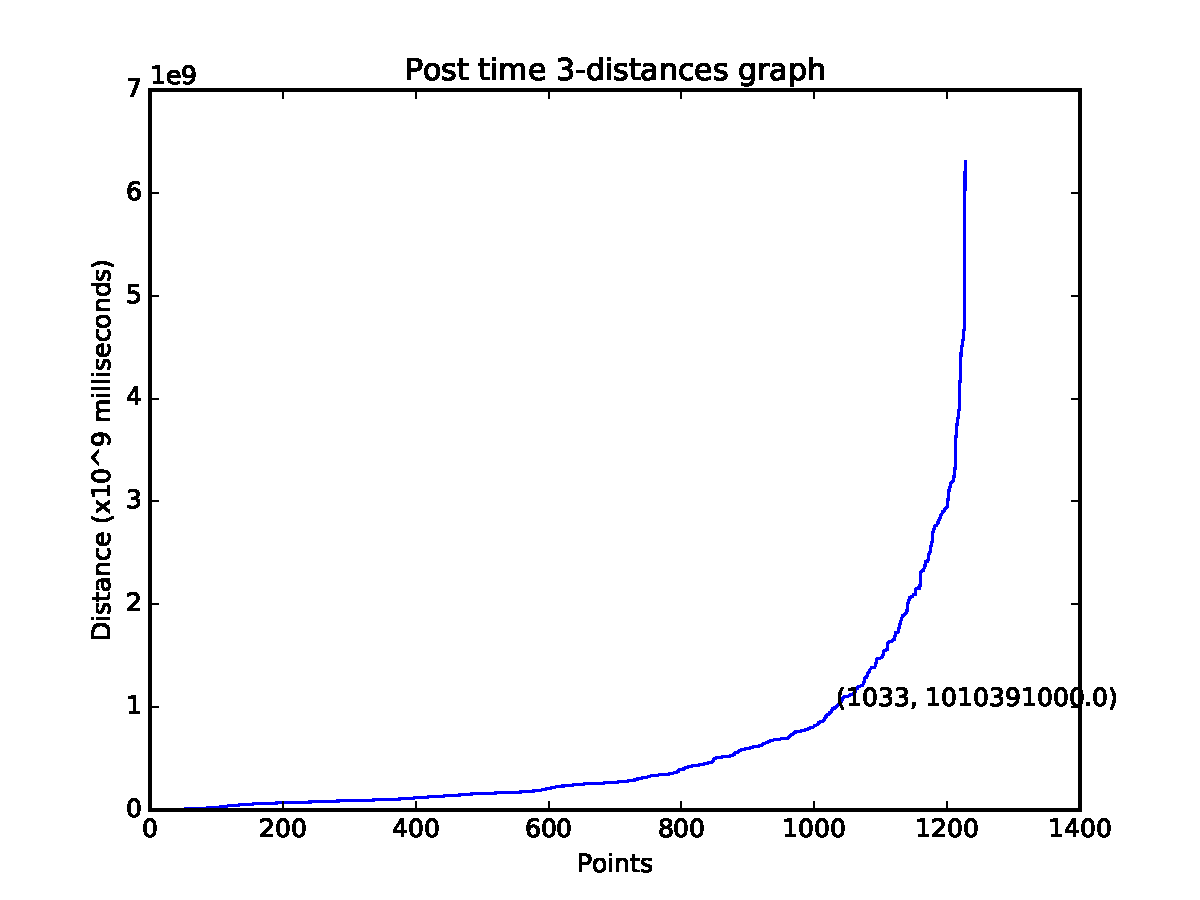
\includegraphics[width=3.5in]{images/post_time_knn.pdf}}
\caption{3-distances graph for post time}
\label{fig:postTime}
\end{figure}
\subsubsection{Generating the question}
The parameter we can choose when generating a question is the length of the time periods proposed to the user. Without difficulty this length is chosen to be proportional to how long in the past the event happened. When incorporating the difficulty we decided to reduce it based on the difficulty: the harder the question has to be, the smaller the time period has to be. We still take into account the date of the event as we have to compensate for the fact that older events are harder to remember.

\subsection{Geolocation Questions}
On this type of question we have nothing to do while generating the question, the selection of an item suffices. Therefore we only need to generate a score for each item. We do it in the same way as for the timeline questions: we cluster the items, an item which is in a cluster will get score 1.0 and an item which is not in a cluster will get score 0.5. The reason for this is that clusters will represent places where the user lives, has lived or goes often so it is easy for them to locate these events as they know the area well. On the other hand the ones outside of a cluster are isolated places and the area is often not known well by the user.\\
For the parameters we used for the DBSCAN clustering, we chose $\minpts$ to be 3 for the reasons expressed in section \ref{subsec:paramselect}. We did not use a 3-distances graph for the choice of $\epsilon$ because there was no user with a satisfying amount of data. So we simply tried different values to see their effect on the clustering and finally decided an $\epsilon$ of 2. This distance is a euclidean distance in the latitude and longitude space.

\subsection{Ordering Questions}
For the ordering questions, as for the geolocation questions, only the items picking matters as there is nothing else to decide when generating the question. There are two types of questions. The first kind is the new question about ordering reactions on a post according to their number on that post. And the second is the questions are the ones about ordering pages according to their number of likes or the time when the user liked the page.
\subsubsection{Reactions ordering}
In this case the difficulty of the question comes from how different the numbers of each reaction are from one another. A good measure for this is the standard deviation, the higher the standard deviation the easiest the question will be. To make sure that this score is between 0 and 1 we first normalize the number of reactions relative to the one with the highest number of reactions, then compute the standard deviation. If we note the standard deviation of the normalized values $\sigma_n$ the difficulty score $\mathit{diffScore}$ will be $$\mathit{diffScore} = 1 - 2 \sigma_n$$ which is between 0 and one as the standard deviation of the normalized values will be between 0 and 0.5.
\subsubsection{Ordering pages}\label{subsubsec:orderpages}
This is an exception to the standard scheme of picking items only based on their score. The difficulty here lies in the similarity between the items, so when we want to generate a hard question we want to select similar items. To decide on the similarity of items we use DBSCAN clustering. We can generate two kind of questions, the hard ones, when the items are selected in the same cluster and the easy ones where the items are selected at random.\\
For the DBSCAN parameters selection we decided to use 3 for $\minpts$ for the reasons mentioned in section \ref{subsec:paramselect}. For the choice of $\epsilon$ we generated 3-distances graphs using the data from a user with a high number of liked pages.\\
For page like times the distances are expressed in milliseconds. Figure \ref{fig:plikeTime} show the resulting graph, we decided to use the value 7709211000 milliseconds for $\epsilon$ which corresponds to approximately 89.22 days.\\
Finally for page like numbers the distances expressed are the distances between the logarithms of the page likes number. As mentioned earlier the number of likes on a page is a power law distribution so using the logarithm of this number makes also sens when clustering. The resulting graph is shown on figure \ref{fig:plikesNumber}. The chosen value for $\epsilon$ is then 0.43349.

\begin{figure}
\centering
{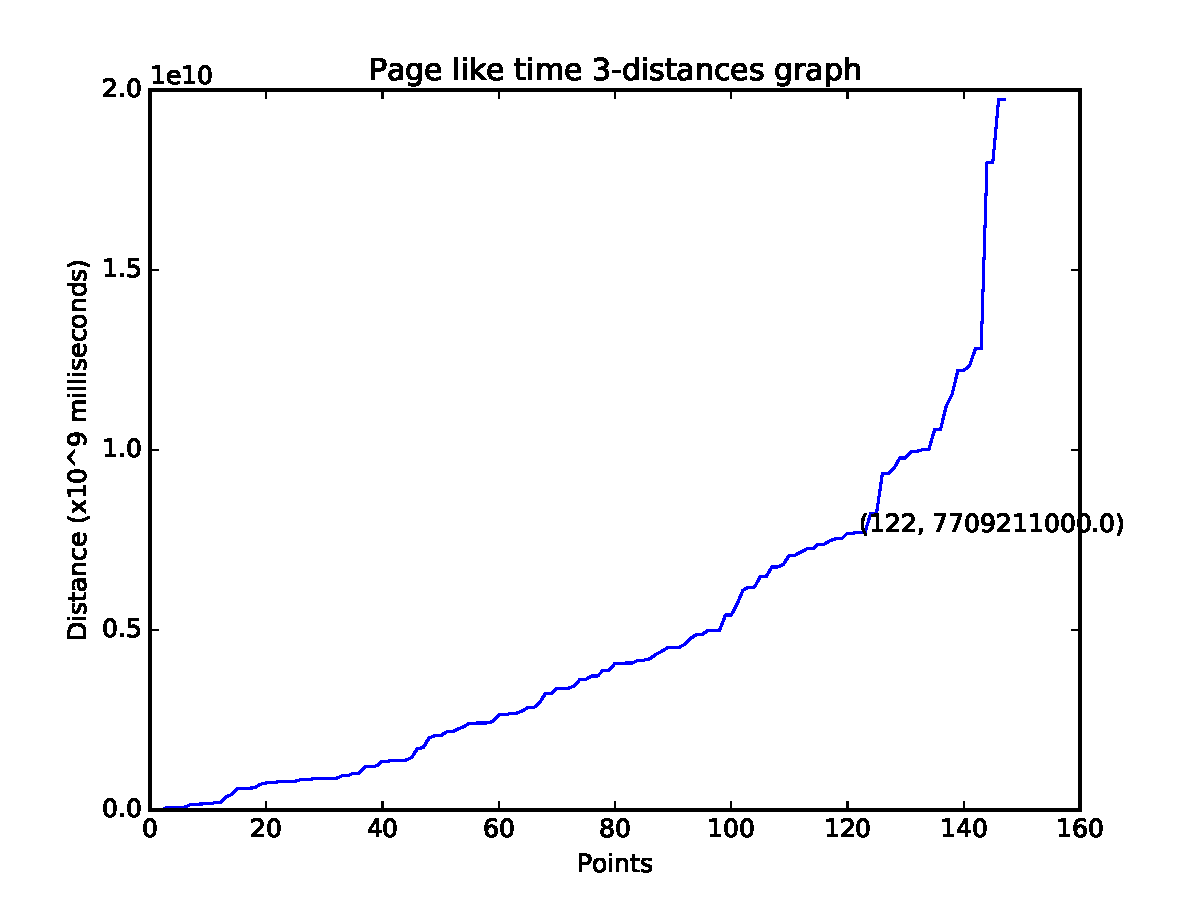
\includegraphics[width=3.5in]{images/page_like_time_knn.pdf}}
\caption{3-distances graph for page like time}
\label{fig:plikeTime}
\end{figure}
\begin{figure}
\centering
{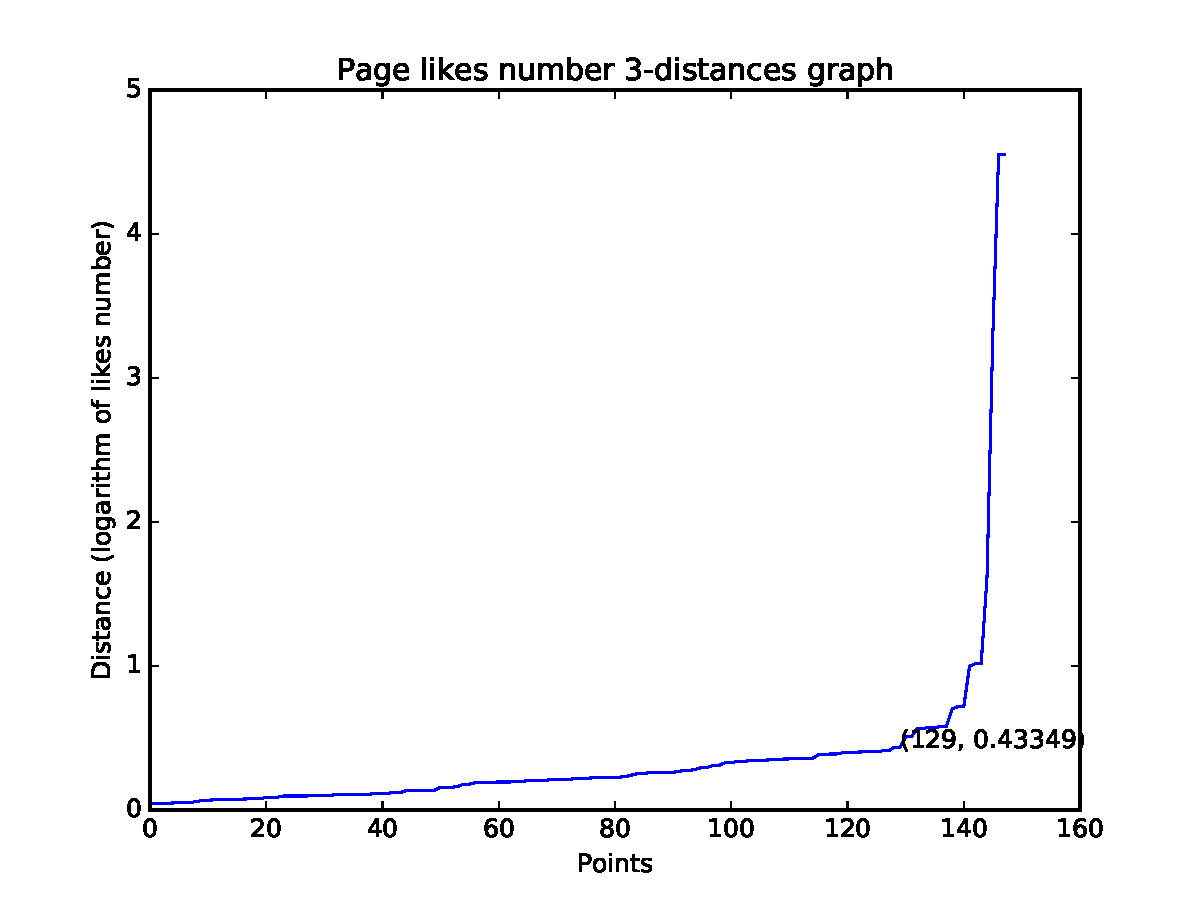
\includegraphics[width=3.5in]{images/page_likes_number_knn.pdf}}
\caption{3-distances graph for page likes number}
\label{fig:plikesNumber}
\end{figure}

\section{Difficulty selection}
The last problem to tackle is choosing the difficulty level we want the questions to be when generating a game board. Thanks to the stats module (see section \ref{sec:stats}) we have easily access to the success rate of a user on any type of question. This success rate being a number between 0 and 1.0 we decided to use this as a measure of required difficulty on any type of question. This means that in the cases where we are trying to generate a question which is not an ordering of pages (we did not compute a score for those, see section \ref{subsubsec:orderpages}) we can simply choose items which score is at least as high as the success rate. This success rate is then also used in the question generation process as a parameter.